\section{Specific Requirements}

\vspace{12pt}

\subsection{External Interface Requirements}

\vspace{12pt}

\subsubsection{User Interfaces}

In this section is presented CKB platform UI. The general view is the same both for educators and students, but there are some small changes between the two views due to additional functions that can be performed by either one or the other. \\ There are some differences that can be detected. For example, an educator must have the possibility to manually evaluate students' projects, while a student can't, or also an educator has the possibility to create a tournament or a battle within a tournament, while a student can't.
\\Nevertheless there are also some common functionalities, such as the option to view tournament rank or the list the ongoing tournaments. 
\\More details in the mockup below.

\vspace{100pt}

\begin{figure}[h]
    \centering
    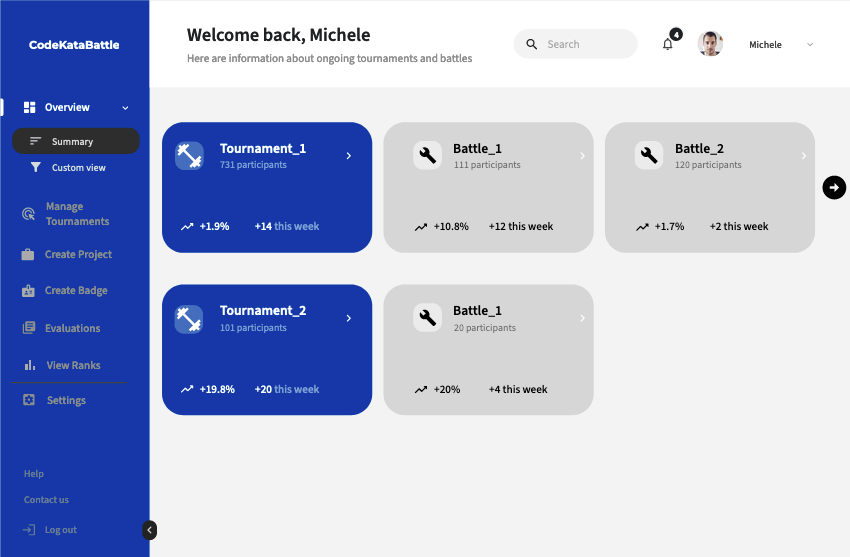
\includegraphics[scale=0.5]{src/educator_view.png}
    \caption*{Educator Interface}
\end{figure} \vspace{0.5cm}

\newpage

In the Educator Interface the main page shows the ongoing tournaments, followed by every ongoing battle for that tournament. \\The search bar allows educator to search for a nickname and find users associated to it, so that it's possible to visualize their profile. \\The main functions an educator can perform are shown on the left column: 
\begin{itemize}
    \item \textbf{Manage Tournaments}: allows an educator to create and close a tournament, create (with all the possible settings) and close battles and eventually grant the permission to create battles to another educator.
    \item \textbf{Create Project}: allows an educator to create a new project to assign to students. 
    \item \textbf{Create Badge}: allows an educator to create a new badge that could be achieved by the students in a tournament.
    \item \textbf{Evaluations}: allows an educator to manually evaluate students' projects.
    \item \textbf{View Ranks}: view all ongoing tournaments and battles rank.
\end{itemize}

\vspace{100pt}

\begin{figure}[h]
    \centering
    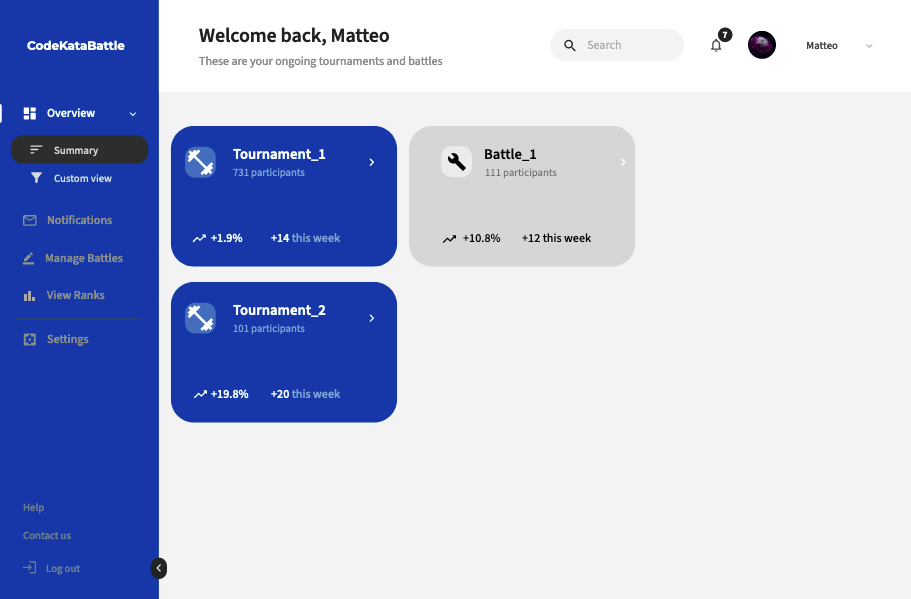
\includegraphics[scale=0.5]{src/student_view.png}
    \caption*{Student Interface}
\end{figure} \vspace{0.5cm}

\newpage

In the Student Interface the main page shows the ongoing tournaments, followed by the battles to which the student is subscribed. \\The search bar allows student to search for a nickname and find users associated to it, so that it's possible to visualize their profile. \\The main functions a student can perform are shown on the left column:
\begin{itemize}
    \item \textbf{Notifications}: allows a student to view the notifications the platform sends when a new tournament or a new battle within a tournament the student is subscribed to is created.
    \item \textbf{Manage Battles}: this section allows a student to create teams and contains the link to the GitHub repository for each battles he/she is subscribed to. 
    \item \textbf{View Ranks}: view all ongoing tournaments and battles rank.
\end{itemize}


\vspace{60pt}

\subsubsection{Hardware Interfaces}

Both educators and students that want to use the system are required to have a personal computer and an internet connection available, because CKB is provided via a web page.

\vspace{20pt}

\subsubsection{Software Interfaces}

The system requires the following software interfaces in order to provide its services. 
\begin{itemize}
    \item \textbf{GitHub API}: the systems has this API to interact with GitHub to detect every push done by each team during a battle. 
\end{itemize}

\vspace{20pt}

\subsubsection{Communication Interfaces}

The system is based on the communication with users' devices and with GitHub application. For the first one, CKB uses internet connection to send and receive data, while for the second one it uses the GitHub API to communicate with GitHub and pull new code sources pushed by students during a battle. 


\newpage

\subsection{Functional Requirements}
In this section are specified the system's requirements, divided in three target groups to better classify them.

\vspace{20pt}

\begin{itemize}
    \item \textbf{Basic Requirements}
    \\
    \\$[R1]$: The systems allows educators to sign up.
    \\$[R2]$: the system allows students to sign up.
    \\$[R3]$: the system allows registered educators to log in.
    \\$[R4]$: the system allows registered students to log in.
    \\
    \item \textbf{Main Requirements} 
    \\
    \\$[R5]$: the system allows educators to create a new tournament.
    \\$[R6]$: the system allows an educator to grant permission to create battles within the context of a specific tournament to another educator.
    \\$[R7]$: the system allows educators to create a new battle, if they have the permission to do it.
    \\$[R8]$: the system notifies all the students subscribed to the platform when a new tournament is created.
    \\$[R9]$: the system allows students to subscribe to a tournament.
    \\$[R10]$: the system notifies all the students subscribed to a specific tournament when a new battle in the context of that tournament is created.
    \\$[R11]$: the system allows educators that created a battle to upload the code kata.
    \\$[R12]$: the system allows educators that created a battle to set minimum and maximum number of students per group.
    \\$[R13]$: the system allows educators that created a battle to set a registration deadline.
    \\$[R14]$: the system allows educators that created a battle to set a final submission deadline.
    \\$[R15]$: the system allows educators that created a battle to set the possibility to manually evaluate projects during the consolidation stage.
    \\$[R16]$: the system allows students to create teams for ongoing battles inviting other students.
    \\$[R17]$: the system allows students to join a battle.
    \\$[R18]$: the system sends to each students that belongs to a team subscribed to a battle the link of the GitHub repository assigned to that team.
    \\$[R19]$: the system allows both students and educators to see the current rank evolving during a battle.
    \\$[R20]$: the system allows educators to manually evaluate projects during the consolidation stage in the context of a specific battle.
    \\$[R21]$: the system notifies all students participating in the battle when the final battle rank becomes available.
    \\$[R22]$: the system allows both educators and students to see the list of ongoing tournaments.
    \\$[R23]$: the system allows both educators and students to see the rank of each ongoing tournament.
    \\$[R24]$: the system allows educators who created a tournament to close it.
    \\$[R25]$: the system notifies all students involved in a tournament when the final rank of that tournament becomes available.
    \\
    \item \textbf{Additional Requirements}
    \\
    \\$[R26]$: the system allows educators that have created a tournament to create badges.
    \\$[R27]$: the system allows both educator and students to visualize the profile and badges of a student.
\end{itemize}

\vspace{40pt}


\subsubsection{Use Cases Diagrams}
In this section, we will provide use case diagrams. Then, for each use case, we will provide a detailed description and a sequence diagram.
\\
\textbf{Note}: in the following diagrams, it is the user who initiates the use case

\vspace{3px}
\begin{figure}[H]
    \centering
    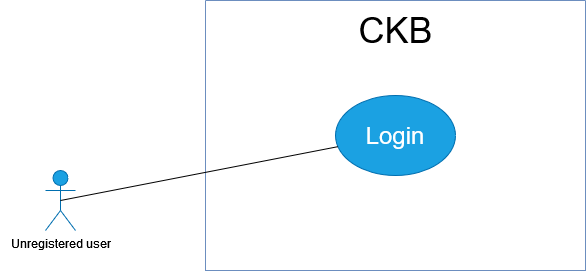
\includegraphics[scale=0.6]{src/uc_diagrams/unregistered_user.png}
    \caption{Unregistered user use case diagram}
\end{figure}

\vspace{3px}
\begin{figure}[H]
    \centering
    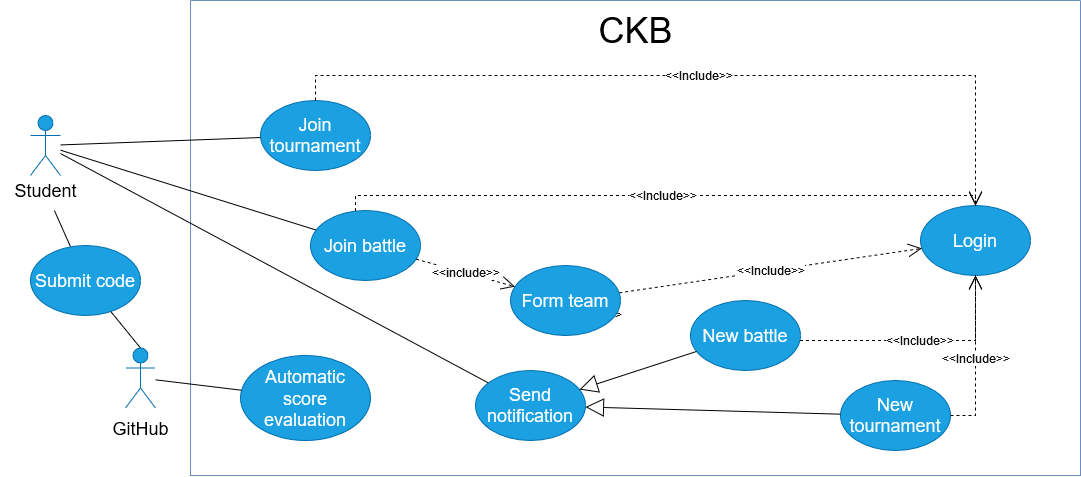
\includegraphics[width=\textwidth]{src/uc_diagrams/student.png}
    \caption{Student use case diagram}
\end{figure}

\vspace{3px}
\begin{figure}[H]
    \centering
    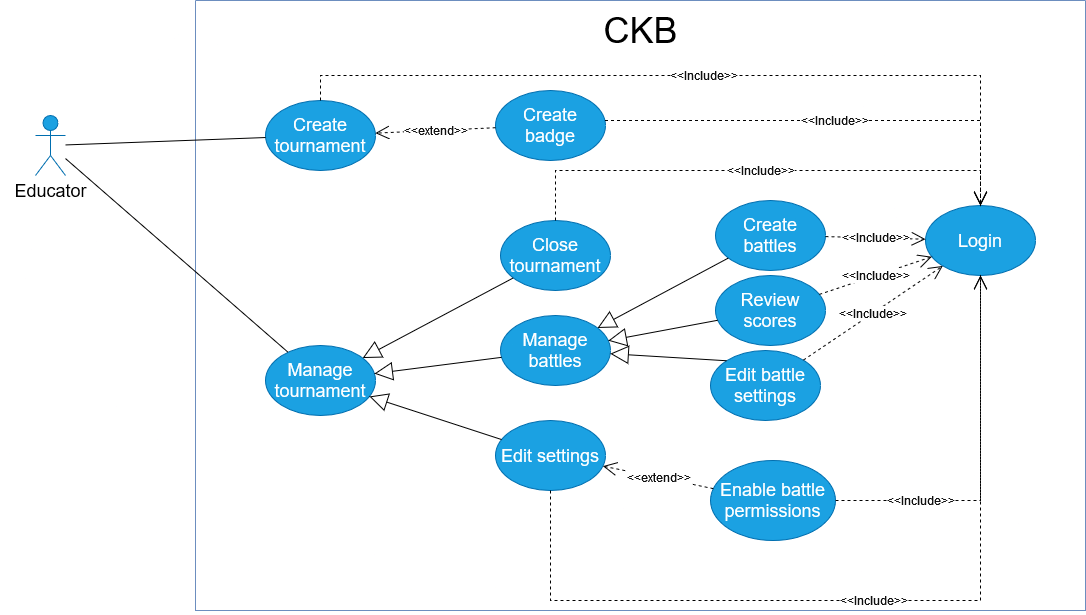
\includegraphics[width=\textwidth]{src/uc_diagrams/educator.png}
    \caption{Educator use case diagram}
\end{figure}

\vspace{3px}
\begin{figure}[H]
    \centering
    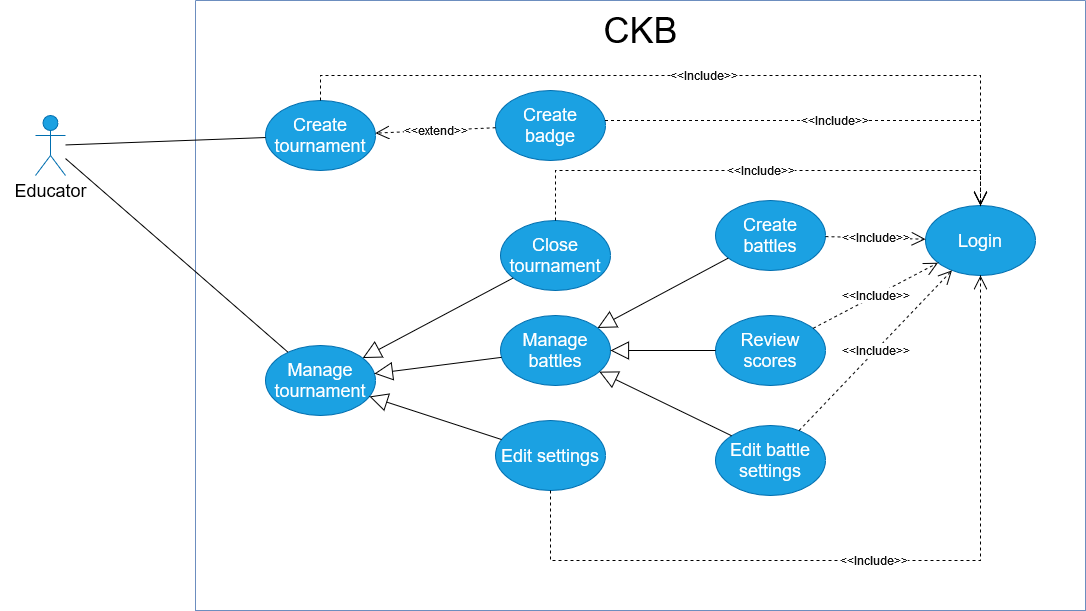
\includegraphics[width=\textwidth]{src/uc_diagrams/generic_user.png}
    \caption{Generic user use case diagram}
\end{figure}

\newpage


\subsubsection{Use Cases}
In the following use cases and sequence diagrams, the system is to be seen as black box interacting with the world.
\usecase
{
    \begin{figure}[H]
        \centering
        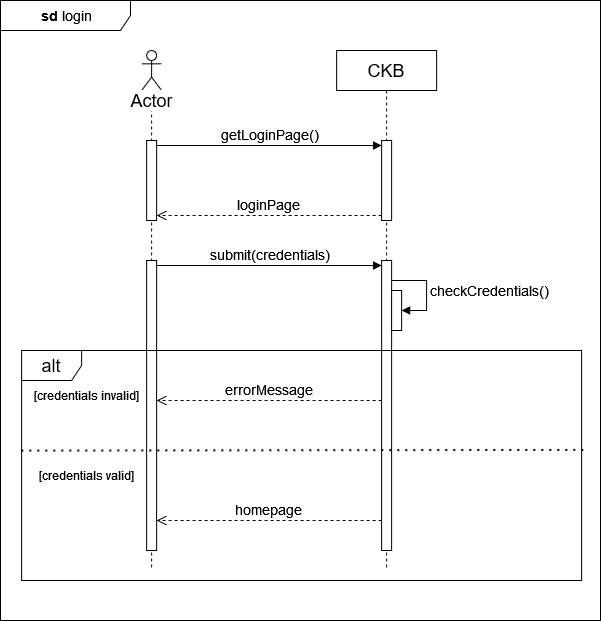
\includegraphics[width=\textwidth]{src/sequence_diagrams/sqlogin.png}
    \end{figure}
}
{1}
{Login}
{User}
{The actor is already registered in the system}
{
    \begin{enumerate}
        \item User requests the Login Page
        \item The system shows the Login Page to user
        \item User inserts credentials and sends them to the system
        \item The system processes the information and shows a success message redirecting the user to the homepage
    \end{enumerate}
}
{User is logged and the homepage is displayed}
{
    \begin{itemize}
        \item A wrong username or password is submitted
    \end{itemize}
}
{
    In case of exception, a human-readable message will be returned by the system.
}

\usecase
{
    \begin{figure}[H]
        \centering
        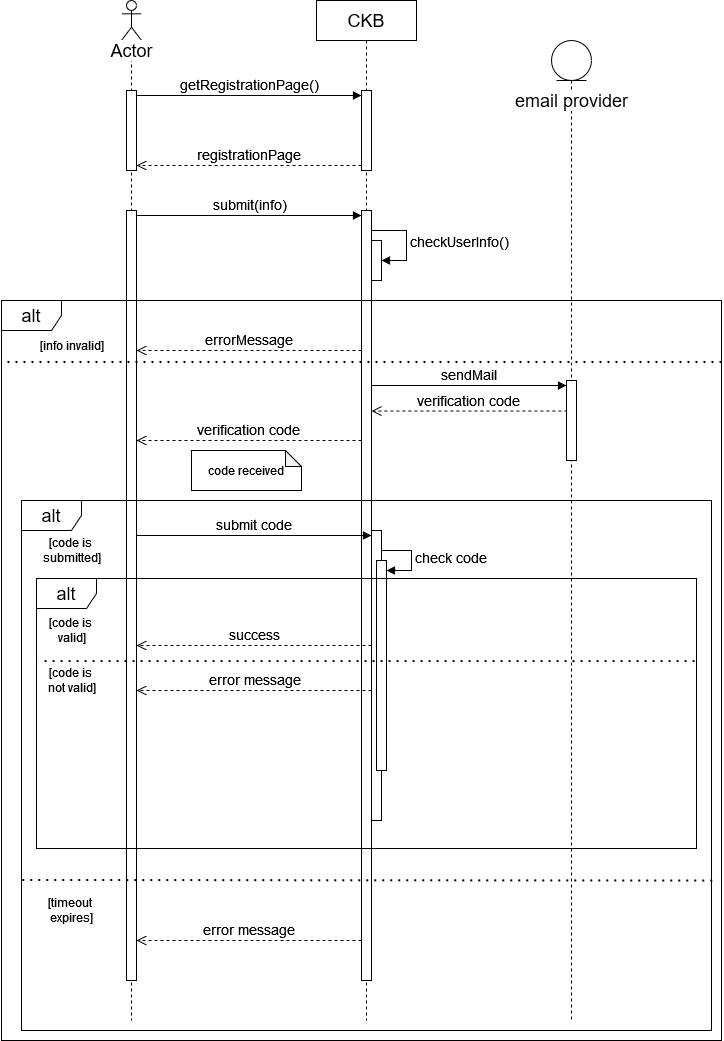
\includegraphics[width=\textwidth]{src/sequence_diagrams/register.png}
    \end{figure}
}
{2}
{User registration} % name
{User, Email provider} % actor
{User clicks 'Sign Up' in the homepage} % entry condition
{ % event flow
    \begin{enumerate}
        \item The system sends user the registration form
        \item User enters email, username password and academic status. Then, submits the data after reading and accepting the Privacy Policy and the Terms of Service
        \item The system sends an email with a secret verification code to Email provider
        \item Email provider receives the email and notifies user
        \item User submits the verification code in the email
        \item The system processes the provided information and displays a success message
    \end{enumerate}
}
{A new account is created} % exit condition
{ % exceptions
    \begin{itemize}
        \item A required registration field is missing when the form is submitted
        \item The username is not available
        \item A wrong verification code is submitted
        \item The timeout for verification expires
    \end{itemize}
}
{ % notes
    All the exceptions above will notify operator with a human-readable message and the system asks to retry
}

\usecase
{
    \begin{figure}[H]
        \centering
        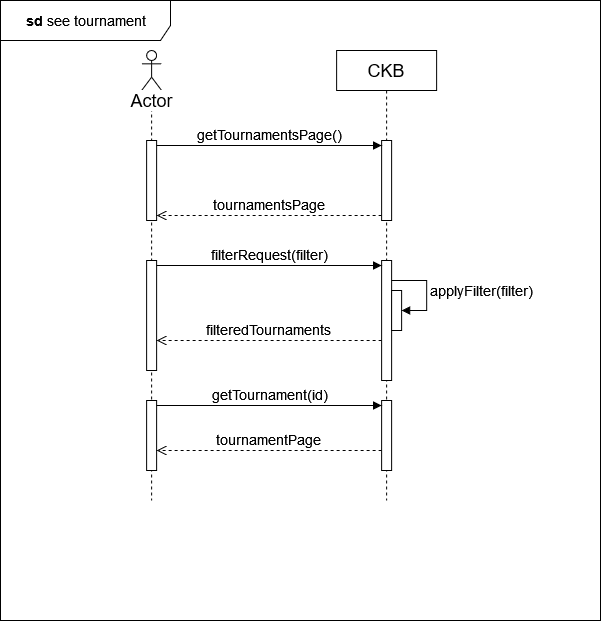
\includegraphics[width=\textwidth]{src/sequence_diagrams/tournaments.png}
    \end{figure}
}
{3}
{See tournament} % name
{User} % actor
{Registered user} % entry condition
{ % event flow
    \begin{enumerate}
        \item User requests to see the tournaments section
        \item The system shows the tournaments section
        \item User applies a filter (ongoing, finished, programming language)    
        \item The system shows the tournaments satisfying the filters
        \item User selects desired tournament
    \end{enumerate}
}
{The system shows the tournament page} % exit condition
{ % exceptions
    None
}
{ % notes
The tournament page displays all the information about that tournament, including rankings, battles and badges
}

\usecase
{
    \begin{figure}[H]
        \centering
        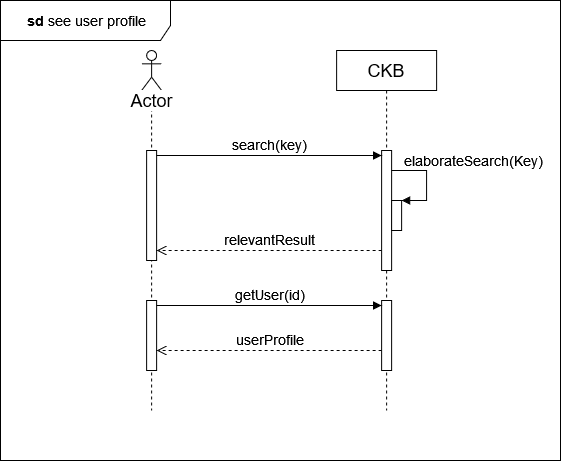
\includegraphics[width=\textwidth]{src/sequence_diagrams/userprofile.png}
    \end{figure}
}
{4}
{See user profile} % name
{User} % actor
{Registered user} % entry condition
{ % event flow
    \begin{enumerate}
        \item User searches a profile by name
        \item The system shows relevant results
        \item User selects the desired profile
    \end{enumerate}
}
{The system shows the profile page} % exit condition
{ % exceptions
    None
}
{ % notes
The profile page displays all the information about a profile, including badges if profile is a student's
}

\usecase
{
    \begin{figure}[H]
        \centering
        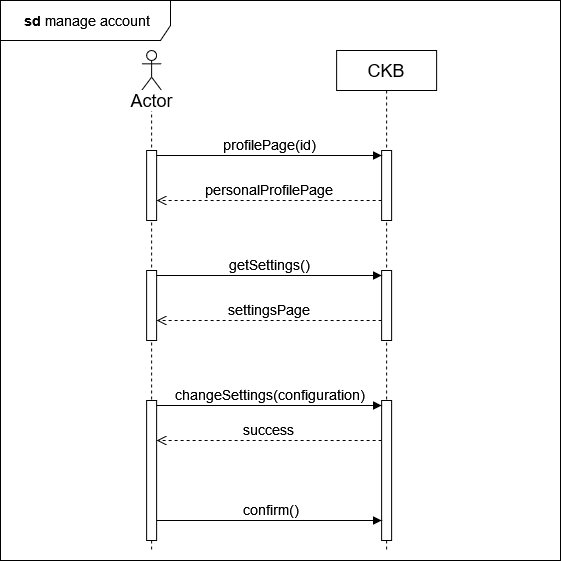
\includegraphics[width=\textwidth]{src/sequence_diagrams/manageaccount.png}
    \end{figure}
}
{5}
{Manage account} % name
{User} % actor
{Registered user} % entry condition
{ % event flow
    \begin{enumerate}
        \item User navigates to personal profile
        \item The system shows the personal profile page
        \item User selects 'change settings'
        \item The system shows the personal settings page
        \item User edits the personal settings to his liking, then clicks confirm
    \end{enumerate}
}
{The system saves the configurations} % exit condition
{ % exceptions
    \begin{itemize}
        \item None
    \end{itemize}
}
{ % notes

}


\usecase
{
    \begin{figure}[H]
        \centering
        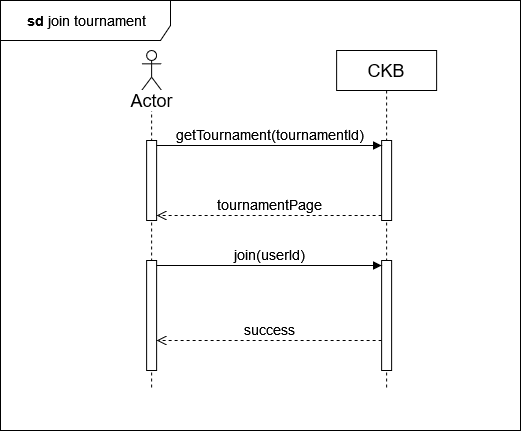
\includegraphics[width=\textwidth]{src/sequence_diagrams/jointourn.png}
    \end{figure}
}
{6}
{Join tournament} % name
{User} % actor
{User logged in to the platform as student, tournament still in subscription phase} % entry condition
{ % event flow
    \begin{enumerate}
        \item User requests the tournament page
        \item The system displays the tournament page
        \item User clicks the 'join' button
    \end{enumerate}
}
{User join the tournament} % exit condition
{ % exceptions
    \begin{itemize}
        \item None
    \end{itemize}
}
{ % notes

}

\usecase
{
    \begin{figure}[H]
        \centering
        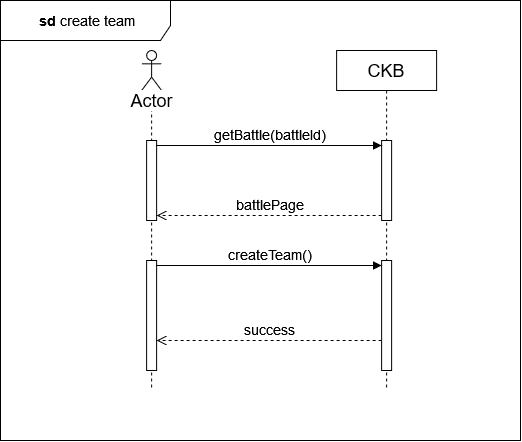
\includegraphics[width=\textwidth]{src/sequence_diagrams/createteam.png}
    \end{figure}
}
{7.1}
{Create team} % name
{User} % actor
{User logged in to the platform as Student, user subscribed to a tournament, the battle is related to that tournament and still in team formation phase, user is not yet part of a team} % entry condition
{ % event flow
    \begin{enumerate}
        \item User navigates to the battle page
        \item The system displays the battle page
        \item User clicks the create team button
    \end{enumerate}
}
{New team is created} % exit condition
{ % exceptions
    \begin{itemize}
        \item None
    \end{itemize}
}
{ % notes
None
}

\usecase
{
    \begin{figure}[H]
        \centering
        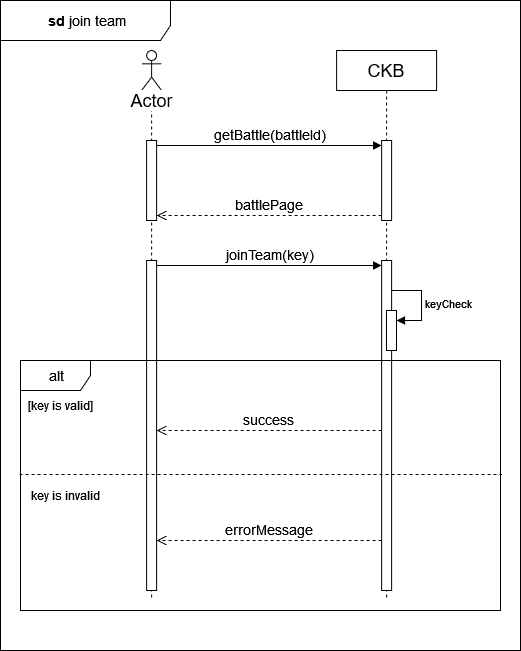
\includegraphics[width=\textwidth]{src/sequence_diagrams/jointeam.png}
    \end{figure}
}
{7.2}
{Join team} % name
{User} % actor
{User logged in to the platform as Student, user subscribed to a tournament, the battle is related to that tournament and still in team formation phase, user is not yet part of a team} % entry condition
{ % event flow
    \begin{enumerate}
        \item User navigates to the battle page
        \item The system displays the battle page
        \item User enters the team code
    \end{enumerate}
}
{User joins team} % exit condition
{ % exceptions
    \begin{itemize}
        \item Team code invalid
    \end{itemize}
}
{ % notes
    \begin{itemize}
        \item The system displays an error message
    \end{itemize}
}

\usecase
{
    \begin{figure}[H]
        \centering
        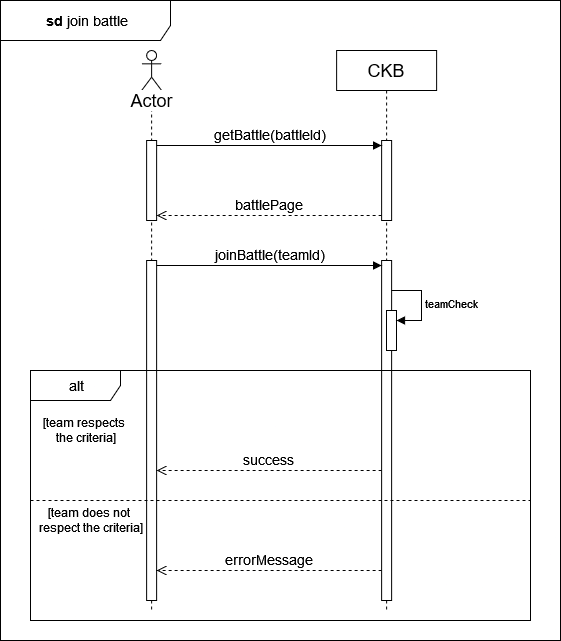
\includegraphics[width=\textwidth]{src/sequence_diagrams/joinbattle.png}
    \end{figure}
}
{7.3}
{Join battle} % name
{User} % actor
{User logged in to the platform as Student, User subscribed to a tournament, the battle is related to that tournament and still in team formation phase, User is the creator of a team} % entry condition
{ % event flow
    \begin{enumerate}
        \item User navigates to the battle page
        \item The system displays the battle page
        \item User clicks join battle
    \end{enumerate}
}
{The team user created joins the battle} % exit condition
{ % exceptions
    \begin{itemize}
        \item The team does not respect the minimum/maximum number of members per team criteria
    \end{itemize}
}
{ % notes
    \begin{itemize}
        \item The system displays an error message and asks to respect the criteria and try again
    \end{itemize}
}


\usecase
{
    {
    \begin{figure}[H]
        \centering
        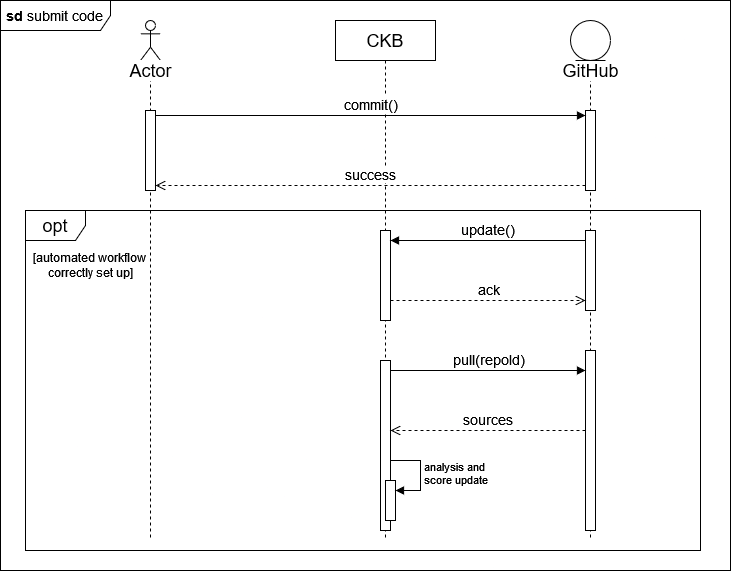
\includegraphics[width=\textwidth]{src/sequence_diagrams/submitcode.png}
    \end{figure}
}
}
{8}
{Submit code} % name
{User, GitHub} % actor
{User logged in to the platform as student, user joined a battle, battle is ongoing} % entry condition
{ % event flow
    \begin{enumerate}
        \item User commits code to main branch on GitHub
        \item GitHub notifies the System through an API call
        \item The system pulls the recent sources from GitHub and evaluates them
    \end{enumerate}
}
{The system shows the updated scores} % exit condition
{ % exceptions
    \begin{itemize}
        \item Student did not set up a proper automated workflow
    \end{itemize}
}
{ % notes
In case of exception, the system will not respond to the new push since It will not be notified
}

\usecase
{
    \begin{figure}[H]
        \centering
        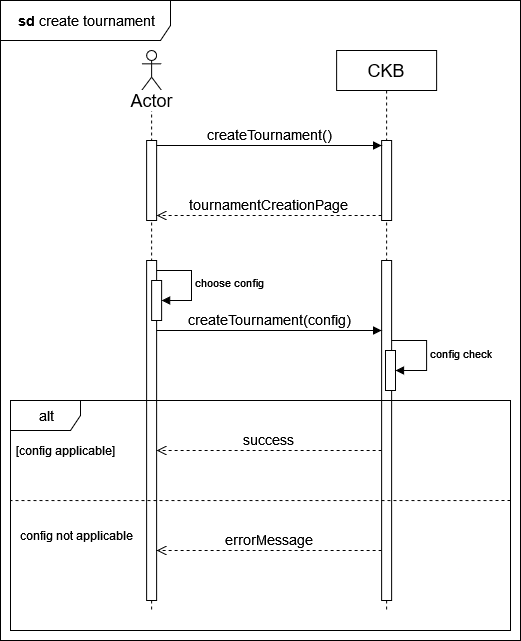
\includegraphics[width=\textwidth]{src/sequence_diagrams/createtourn.png}
    \end{figure}
}
{9}
{Create tournament} % name
{User} % actor
{User logged in to the platform as Educator} % entry condition
{ % event flow
    \begin{enumerate}
        \item User clicks the create tournament button
        \item The system shows the create torunament page
        \item User chooses his desired settings for that tournament, (including name, deadlines, badges, educators allowed to create battles, ...), then submits
    \end{enumerate}
}
{New tournament is created} % exit condition
{ % exceptions
    \begin{itemize}
        \item One or more of the settings is not applicable
    \end{itemize}
}
{ % notes
    \begin{itemize}
        \item Exception: the system displays a message showing the issue and asking to address It before trying again
    \end{itemize}
    User can choose his desired settings here, but he will be able to edit some of them even after tournament creation
}

\usecase
{
    \begin{figure}[H]
        \centering
        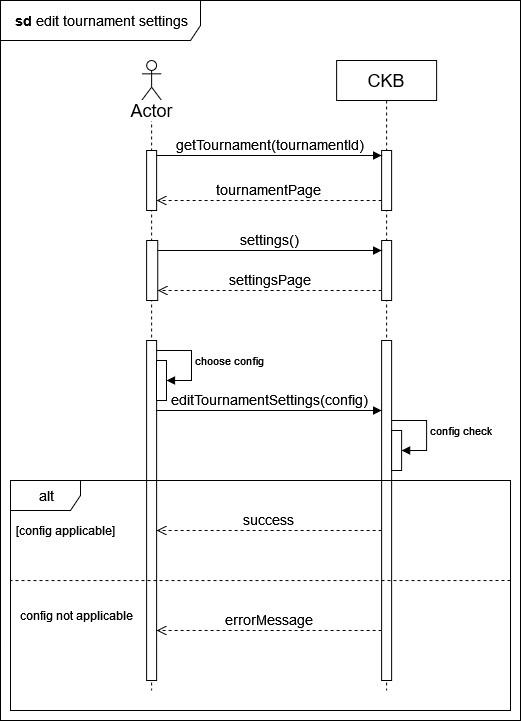
\includegraphics[width=\textwidth]{src/sequence_diagrams/managetournsetts.png}
    \end{figure}
}
{10}
{Edit tournament settings} % name
{User} % actor
{User logged in to the platform as educator, the tournament is not closed, user is the owner of the tournament} % entry condition
{ % event flow
    \begin{enumerate}
        \item User navigates to the tournament page
        \item The system shows the tournament page
        \item User goes to the settings section
        \item The system shows the settings page
        \item User chooses his desired settings, then submits
    \end{enumerate}
}
{Tournament settings are updated} % exit condition
{ % exceptions
    \begin{itemize}
        \item One or more of the settings is not applicable
    \end{itemize}
}
{ % notes
    \begin{itemize}
        \item Exception: the system displays a message showing the issue and asking to address It before trying again
    \end{itemize}
}

\usecase
{
    \begin{figure}[H]
        \centering
        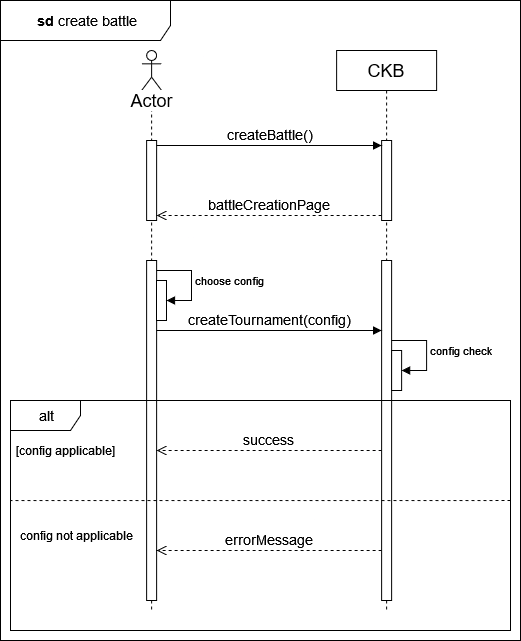
\includegraphics[width=\textwidth]{src/sequence_diagrams/createbattle.png}
    \end{figure}
}
{11.1}
{Create battle} % name
{User} % actor
{User logged in to the platform as educator, tournament is ongoing, user has been granted permission to create battles (or is the tournament creator itself)} % entry condition
{ % event flow
    \begin{enumerate}
        \item User navigates to the tournament page
        \item The system displays the tournament page
        \item User clicks the create new battle button
        \item The system shows the battle creation page
        \item User chooses his desired settings (like uploading code kata,            setting minimum and maximum number of students per team,                deadlines, ...) and submits
    \end{enumerate}
}
{New battle is created within the context of that tournament} % exit condition
{ % exceptions
    \begin{itemize}
        \item One or more of the settings is not applicable
    \end{itemize}
}
{ % notes
    \begin{itemize}
        \item Exception: the system displays a message showing the issue and asking to address It before trying again
    \end{itemize} 
    User can choose his desired settings here, but he will be able to edit some of them even after battle creation
}

\usecase
{
    \begin{figure}[H]
        \centering
        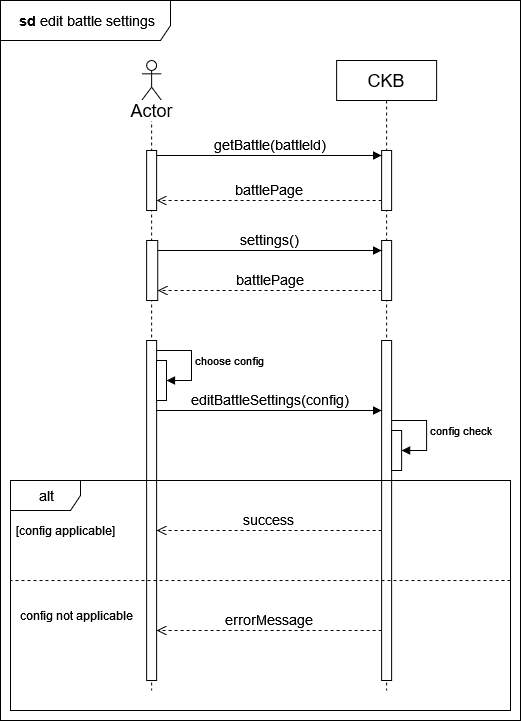
\includegraphics[width=\textwidth]{src/sequence_diagrams/managebattsetts.png}
    \end{figure}
}
{11.2}
{Edit battle settings} % name
{User} % actor
{User logged in to the platform as educator, battle is ongoing, user has been granted permission to create battles (or is the tournament creator itself)} % entry condition
{ % event flow
    \begin{enumerate}
        \item User navigates to the battle page
        \item User clicks the edit settings button
        \item The system shows the settings section
        \item User chooses his desired settings and submits
    \end{enumerate}
}
{Battle configurations are updated} % exit condition
{ % exceptions
    \begin{itemize}
        \item One or more of the settings is not applicable
    \end{itemize}
}
{ % notes
    \begin{itemize}
        \item Exception: the system displays a message showing the issue and asking to address It before trying again
    \end{itemize}
}

\usecase
{
    \begin{figure}[H]
        \centering
        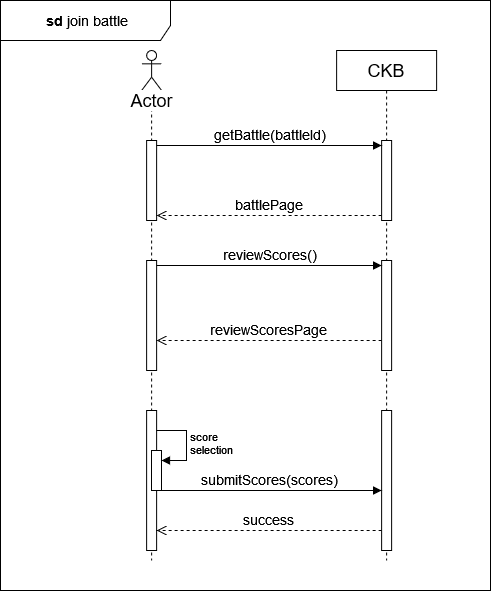
\includegraphics[width=\textwidth]{src/sequence_diagrams/revscores.png}
    \end{figure}
}
{11.3}
{Review scores} % name
{User} % actor
{User logged in to the platform as educator, battle is in consolidation phase, user has been granted permission to create battles (or is the tournament creator itself)} % entry condition
{ % event flow
    \begin{enumerate}
        \item User navigates to the battle page
        \item User clicks the review scores button
        \item The system shows the review scores section
        \item User performs manual evaluation, then submits
    \end{enumerate}
}
{Battle scores are updated} % exit condition
{ % exceptions
    \begin{itemize}
        \item None
    \end{itemize}
}
{ % notes

}

\usecase
{
    \begin{figure}[H]
        \centering
        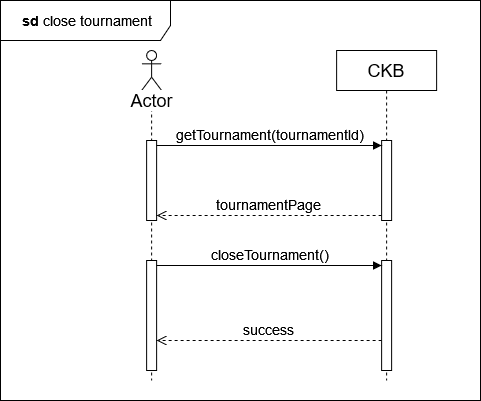
\includegraphics[width=\textwidth]{src/sequence_diagrams/closetourn.png}
    \end{figure}
}
{12}
{Close tournament} % name
{User} % actor
{User logged in to the platform as educator, tournament is ongoing, user is tournament creator} % entry condition
{ % event flow
    \begin{enumerate}
        \item User navigates to the tournament page
        \item The system shows the tournament page
        \item User clicks close tournament button
    \end{enumerate}
}
{Tournament is closed} % exit condition
{ % exceptions
    \begin{itemize}
        \item None
    \end{itemize}
}
{ % notes

}

\usecase
{
    \begin{figure}[H]
        \centering
        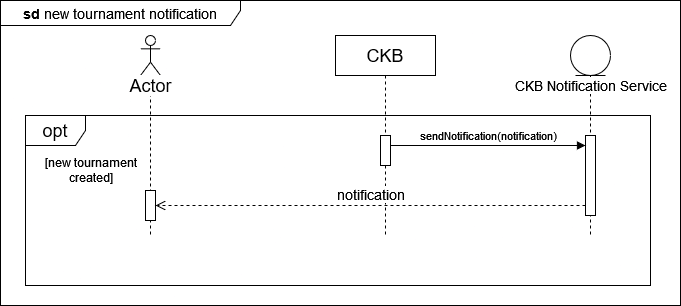
\includegraphics[width=\textwidth]{src/sequence_diagrams/notifytourn.png}
    \end{figure}
}
{13.1}
{New tournament notification} % name
{User, CKB Notification Service} % actor
{User logged in to the platform as student} % entry condition
{ % event flow
    \begin{enumerate}
        \item New tournament is created in the platform
        \item The system calls the CKB Notification Service
        \item CKB Notification Service sends the notification
    \end{enumerate}
}
{User is notified} % exit condition
{ % exceptions
    \begin{itemize}
        \item None
    \end{itemize}
}
{ % notes

}

\usecase
{
    \begin{figure}[H]
        \centering
        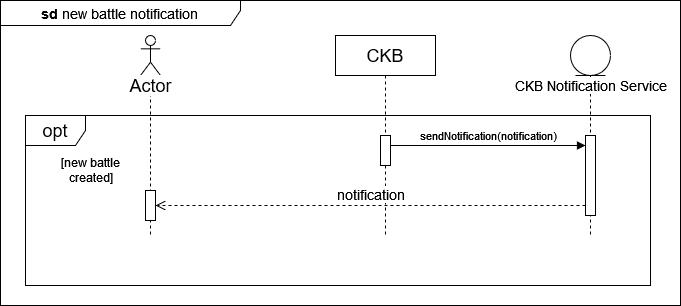
\includegraphics[width=\textwidth]{src/sequence_diagrams/notifybattle.png}
    \end{figure}
}
{13.2}
{New battle notification} % name
{User, CKB Notification Service} % actor
{User logged in to the platform as student, User subscribed to a tournament} % entry condition
{ % event flow
    \begin{enumerate}
        \item New battle is created in the context of a tournament user is subscribed to
        \item The system calls the CKB Notification Service
        \item CKB Notification Service sends the notification
    \end{enumerate}
}
{User is notified} % exit condition
{ % exceptions
    \begin{itemize}
        \item None
    \end{itemize}
}
{ % notes

}

\usecase
{
    \begin{figure}[H]
        \centering
        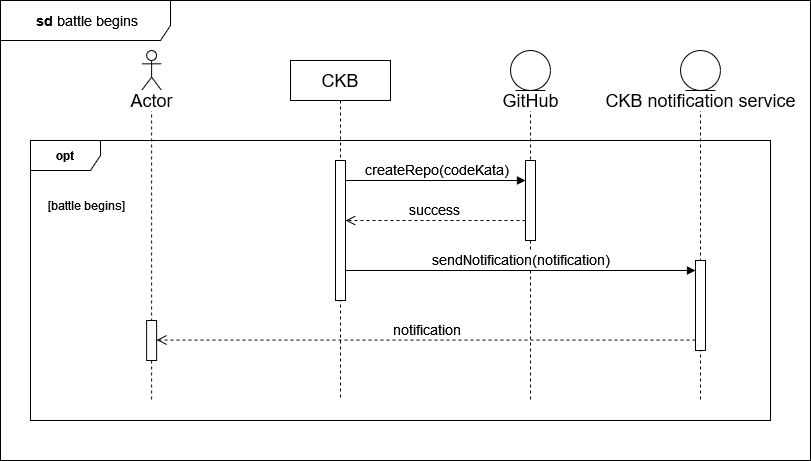
\includegraphics[width=\textwidth]{src/sequence_diagrams/battlebegins.png}
    \end{figure}
}
{13.3}
{Battle begins notification} % name
{User, CKB Notification Service, GitHub} % actor
{User logged in to the platform as student, User subscribed to a tournament, user joined a battle} % entry condition
{ % event flow
    \begin{enumerate}
        \item Battle team formation deadline expires, battle begins
        \item The system creates a new GitHub repository containing the codekata
        \item GitHub successfully creates the repository 
        \item The system calls the CKB Notification Service 
        \item CKB Notification Service sends the notification
    \end{enumerate}
}
{User receives the notification and the link to the github repository} % exit condition
{ % exceptions
    \begin{itemize}
        \item None
    \end{itemize}
}
{ % notes

}

\usecase
{
    \begin{figure}[H]
        \centering
        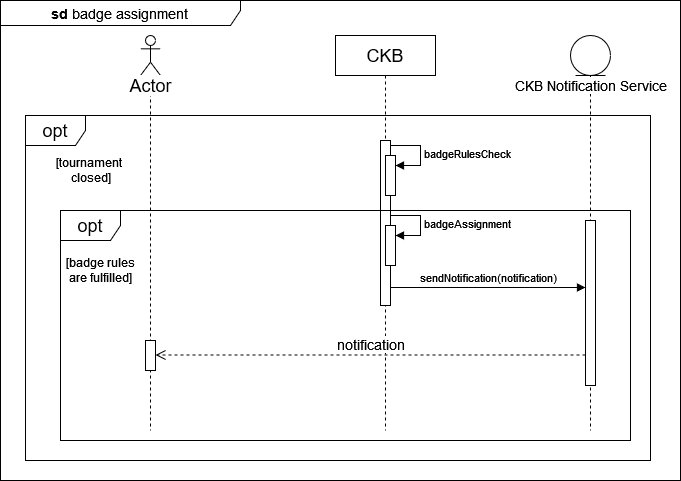
\includegraphics[width=\textwidth]{src/sequence_diagrams/badgeassignment.png}
    \end{figure}
}
{14}
{Badges assignment} % name
{User, CKB Notification Service} % actor
{User subscribed to a tournament, tournament has a badge associated} % entry condition
{ % event flow
    \begin{enumerate}
        \item Tournament is closed
        \item The system checks the badge rules fulfillment for all students subscribed to that tournament
        \item User is assigned a badge
        \item The system calls the CKB Notification Service 
        \item CKB Notification Service sends the notification
    \end{enumerate}
}
{User receives the notification of the badge assigned} % exit condition
{ % exceptions
    \begin{itemize}
        \item User does not fulfill the rules associated to the badge
    \end{itemize}
}
{ % notes
    \begin{itemize}
        \item Exception: User is not assigned the badge, thus does not receive the notification
    \end{itemize}
    This operation is performed for every badge associated with the tournament that is closed
}




\newpage

\subsubsection{Requirements Mapping}

\vspace{1cm}

\begin{table}[H]
    \centering
    \begin{tabular}{|p{8cm}|p{8cm}|}
      \hline
      \multicolumn{2}{|p{16cm}|}{\textbf{$[G1]$ Educator can manage (create battles and badges, grant permission to other Educators, and close) each tournament he/she creates. }} \\
      \hline
      {$[R1]$: The systems allows educators to sign up.
      \newline$[R3]$: the system allows registered educators to log in.
      \newline$[R5]$: the system allows educators to create a new tournament.
      \newline$[R6]$: the system allows an educator to grant permission to create battles within the context of a specific tournament to another educator.
      \newline$[R7]$: the system allows educators to create a new battle, if they have the permission to do it.
      \newline$[R24]$: the system allows educators who created a tournament to close it.
      \newline$[R26]$: the system allows educators that have created a tournament to create badges.}
      & 
      {$[D1]$: Users have reliable and consistent access to the internet to participate in code kata battles and interact with the platform.
      \newline$[D2]$: Users have access to suitable devices, such as computers or mobile devices, with compatible web browsers.
      \newline$[D3]$: Educators have a basic understanding of the CodeKataBattle platform's features, enabling them to create and manage tournaments and battles effectively. In particular, they have to provide correct tests and rules for projects and badges.
      \newline$[D5]$: User-provided data, including user profiles, code submissions, and scoring information, is assumed to be accurate and valid. Users are supposed to providing truthful information.
      \newline$[D7]$: The platform assumes a high level of system uptime, with minimal downtime, to support user interactions, database storage, and real-time features.
      \newline$[D9]$: Users are responsible for maintaining the security and privacy of their accounts, including choosing strong passwords and keeping their login credentials confidential.}
      \\
      \hline
    \end{tabular}
\end{table}

\begin{table}[H]
    \centering
\begin{tabular}{|p{8cm}|p{8cm}|}
  \hline
  \multicolumn{2}{|p{16cm}|}{\textbf{$[G2]$ Educator can manage (deliver exercise, set options, evaluate teams submissions and check rank) each battle he/she creates.}} \\
  \hline
  {
  $[R1]$: The systems allows educators to sign up.
  \newline$[R3]$: the system allows registered educators to log in.
  \newline$[R11]$: the system allows educators that created a battle to upload the code kata.
  \newline$[R12]$: the system allows educators that created a battle to set minimum and maximum number of students per group.
  \newline$[R13]$: the system allows educators that created a battle to set a registration deadline.    \newline$[R14]$: the system allows educators that created a battle to set a final submission deadline.
  \newline$[R15]$: the system allows educators that created a battle to set the possibility to manually evaluate projects during the consolidation stage.
  \newline$[R19]$: the system allows both students and educators to see the current rank evolving during a battle.
  \newline$[R20]$: the system allows educators to manually evaluate projects during the consolidation stage in the context of a specific battle.
  }
  & 
  {
  $[D1]$: Users have reliable and consistent access to the internet to participate in code kata battles and interact with the platform.
  \newline$[D2]$: Users have access to suitable devices, such as computers or mobile devices, with compatible web browsers.
  \newline$[D3]$: Educators have a basic understanding of the CodeKataBattle platform's features, enabling them to create and manage tournaments and battles effectively. In particular, they have to provide correct tests and rules for projects and badges. 
  \newline$[D5]$: User-provided data, including user profiles, code submissions, and scoring information, is assumed to be accurate and valid. Users are supposed to providing truthful information.
  \newline$[D7]$: The platform assumes a high level of system uptime, with minimal downtime, to support user interactions, database storage, and real-time features.
  \newline$[D9]$: Users are responsible for maintaining the security and privacy of their accounts, including choosing strong passwords and keeping their login credentials confidential.
  }
  \\
  \hline
\end{tabular}
\end{table}

\begin{table}[H]
    \centering
\begin{tabular}{|p{8cm}|p{8cm}|}
  \hline
  \multicolumn{2}{|p{16cm}|}{\textbf{$[G3]$ Student can subscribe to a tournament.}} \\
  \hline
  {
  $[R2]$: the system allows students to sign up.
  \newline$[R4]$: the system allows registered students to log in.
  \newline$[R8]$: the system notifies all the students subscribed to the platform when a new tournament is created.
  \newline$[R9]$: the system allows students to subscribe to a tournament.
  }
  & 
  {
  $[D1]$: Users have reliable and consistent access to the internet to participate in code kata battles and interact with the platform.
  \newline$[D2]$: Users have access to suitable devices, such as computers or mobile devices, with compatible web browsers.
  \newline$[D5]$: User-provided data, including user profiles, code submissions, and scoring information, is assumed to be accurate and valid. Users are supposed to providing truthful information.
  \newline$[D7]$: The platform assumes a high level of system uptime, with minimal downtime, to support user interactions, database storage, and real-time features.
  \newline$[D9]$: Users are responsible for maintaining the security and privacy of their accounts, including choosing strong passwords and keeping their login credentials confidential.
  }
  \\
  \hline
\end{tabular}
\end{table}

\begin{table}[H]
    \centering
\begin{tabular}{|p{8cm}|p{8cm}|}
  \hline
  \multicolumn{2}{|p{16cm}|}{\textbf{$[G4]$ Student can manage (subscribe and check rank) their participation to a battle.}} \\
  \hline
  {
  $[R2]$: the system allows students to sign up.
  \newline$[R4]$: the system allows registered students to log in.
  \newline$[R10]$: the system notifies all the students subscribed to a specific tournament when a new battle in the context of that tournament is created.
  \newline$[R16]$: the system allows students to create teams for ongoing battles inviting other students.
  \newline$[R17]$: the system allows students to join a battle.
  \newline$[R18]$: the system sends to each students that belongs to a team subscribed to a battle the link of the GitHub repository assigned to that team.
  \newline$[R19]$: the system allows both students and educators to see the current rank evolving during a battle.
  \newline$[R21]$: the system notifies all students participating in the battle when the final battle rank becomes available.
  }
  & 
  {
  $[D1]$: Users have reliable and consistent access to the internet to participate in code kata battles and interact with the platform.
  \newline$[D2]$: Users have access to suitable devices, such as computers or mobile devices, with compatible web browsers.
  \newline$[D4]$: Students know how to configure Github Actions for let the system aware of the push on the main branch.
  \newline$[D5]$: User-provided data, including user profiles, code submissions, and scoring information, is assumed to be accurate and valid. Users are supposed to providing truthful information.
  \newline$[D6]$: Users will use the platform responsibly, adhering to ethical guidelines and academic integrity. Students are expected to complete code katas independently or within the rules of team collaboration defined by educators.
  \newline$[D7]$: The platform assumes a high level of system uptime, with minimal downtime, to support user interactions, database storage, and real-time features.
  \newline$[D8]$: Some platform functionalities may rely on external services, such as email verification, communication tools and Github integrations.
  \newline$[D9]$: Users are responsible for maintaining the security and privacy of their accounts, including choosing strong passwords and keeping their login credentials confidential.
  \newline$[D10]$: Users are expected to engage in ethical behavior, respecting intellectual property rights, academic integrity, and community guidelines established by the platform.
  }
  \\
  \hline
\end{tabular}
\end{table}

\begin{table}[H]
    \centering
\begin{tabular}{|p{8cm}|p{8cm}|}
  \hline
  \multicolumn{2}{|p{16cm}|}{\textbf{$[G5]$ Both educators and students can check rank for each tournament.}} \\
  \hline
  {
  $[R1]$: The systems allows educators to sign up.
  \newline$[R2]$: the system allows students to sign up.
  \newline$[R3]$: the system allows registered educators to log in.
  \newline$[R4]$: the system allows registered students to log in.
  \newline$[R23]$: the system allows both educators and students to see the rank of each ongoing tournament.
  \newline$[R25]$: the system notifies all students involved in a tournament when the final rank of that tournament becomes available.
  }
  & 
  {
  $[D1]$: Users have reliable and consistent access to the internet to participate in code kata battles and interact with the platform.
  \newline$[D2]$: Users have access to suitable devices, such as computers or mobile devices, with compatible web browsers.
  \newline$[D5]$: User-provided data, including user profiles, code submissions, and scoring information, is assumed to be accurate and valid. Users are supposed to providing truthful information.
  \newline$[D7]$: The platform assumes a high level of system uptime, with minimal downtime, to support user interactions, database storage, and real-time features.
  \newline$[D9]$: Users are responsible for maintaining the security and privacy of their accounts, including choosing strong passwords and keeping their login credentials confidential.
  }
  \\
  \hline
\end{tabular}
\end{table}

\begin{table}[H]
  \centering
\begin{tabular}{|p{8cm}|p{8cm}|}
  \hline
  \multicolumn{2}{|p{16cm}|}{\textbf{$[G6]$ Both educators and students can visualize the profile of a Student.}} \\
  \hline
  {
  $[R1]$: The systems allows educators to sign up.
  \newline$[R2]$: the system allows students to sign up.
  \newline$[R3]$: the system allows registered educators to log in.
  \newline$[R4]$: the system allows registered students to log in.
  \newline$[R27]$: the system allows both educator and students to visualize the profile and badges of a student.
  }
  & 
  {
  $[D1]$: Users have reliable and consistent access to the internet to participate in code kata battles and interact with the platform.
  \newline$[D2]$: Users have access to suitable devices, such as computers or mobile devices, with compatible web browsers.
  \newline$[D5]$: User-provided data, including user profiles, code submissions, and scoring information, is assumed to be accurate and valid. Users are supposed to providing truthful information.
  \newline$[D7]$: The platform assumes a high level of system uptime, with minimal downtime, to support user interactions, database storage, and real-time features.
  \newline$[D9]$: Users are responsible for maintaining the security and privacy of their accounts, including choosing strong passwords and keeping their login credentials confidential.
  }
  \\
  \hline
\end{tabular}
\end{table}

\begin{table}[H]
\begin{tabular}{|p{8cm}|p{8cm}|}
  \hline
  \multicolumn{2}{|p{16cm}|}{\textbf{$[G7]$ Both educators and students can see the list of ongoing tournaments.}} \\
  \hline
  {
  $[R1]$: The systems allows educators to sign up.
  \newline$[R2]$: the system allows students to sign up.
  \newline$[R3]$: the system allows registered educators to log in.
  \newline$[R4]$: the system allows registered students to log in.
  \newline$[R22]$: the system allows both educators and students to see the list of ongoing tournaments.
  }
  & 
  {
  $[D1]$: Users have reliable and consistent access to the internet to participate in code kata battles and interact with the platform.
  \newline$[D2]$: Users have access to suitable devices, such as computers or mobile devices, with compatible web browsers.
  \newline$[D5]$: User-provided data, including user profiles, code submissions, and scoring information, is assumed to be accurate and valid. Users are supposed to providing truthful information.
  \newline$[D7]$: The platform assumes a high level of system uptime, with minimal downtime, to support user interactions, database storage, and real-time features.
  \newline$[D9]$: Users are responsible for maintaining the security and privacy of their accounts, including choosing strong passwords and keeping their login credentials confidential.
  }
  \\
  \hline
\end{tabular}
\end{table}










\newpage

\subsection{Performance Requirements}

To work properly the system must guarantee low response time in some aspects such as the time spent to calculate and update the battle score of each team after a pull of the latest sources by the platform. \\ Another aspect that must be prioritized is the deadline management to avoid some users perform actions out of the maximum time estabilished, such as subscription to a battle or push new code on GitHub. Moreover, the system has to send as soon as possible the notifications that have to be sent to students. \\However there could be problems out of the system that can affect the performances, for example problems with users' devices or their internet connection.


\vspace{50pt}

\subsection{Design Constraints}

\vspace{20pt}

\subsubsection{Standards compliance}
In the development of CKB several standards and compliance considerations are addressed. The wireless network communication adheres to the IEEE 802.11 standard, ensuring a reliable and secure connection for users participating in coding challenges. Additionally, strict adherence to data protection standards is paramount, with the implementation of privacy laws and regulations governing the handling of personal information.
\\To facilitate collaboration and version control in the development process, the system integrates the Git protocol for communication with GitHub, following established best practices for code repository management.
\\Given the competitive coding nature of the platform, it is imperative to align with OWASP guidelines for web application security. This encompasses robust measures to prevent common vulnerabilities, secure coding practices, and continuous monitoring to ensure the highest standards of security in the challenges and user interactions.
\\Furthermore, considering the dynamic nature of the platform and its coding challenges, accessibility standards (such as WCAG) are implemented to guarantee an inclusive experience for users. Additionally, performance standards are upheld to ensure the website's responsiveness and optimal user experience across various devices and network conditions. 

\vspace{20pt}

\subsubsection{Hardware limitations}

There are very few hardware requirements to use the platform. Users shall have an internet connection (Wi-Fi) and a modern device. 

\vspace{20pt}

\subsubsection{Any other constraint}

There are no limitiations about users, everyone can sign in to CKB and try its functionalities. To facilitate interactions with users the application page should be intuitive, simple to interact with and aesthetically pleasing.


\newpage

\subsection{Software System Attributes}

\vspace{20pt}

\subsubsection{Reliability}

CKB should exhibit consistent and predictable performance, minimizing the occurrence of failures or disruptions, and ensuring its ability to deliver intended functionality over time.
According to this, the system is distributed and its data are replicated in order to guarantee continuous interactions with it.  

\vspace{20pt}

\subsubsection{Availabilty}

There is no constraint about the time during the day the system can be accessed, so it has to be online as much time as possible. In particular CKB must guarantee availability of 99.9\% so that users are affected by offline periods as less as possible.

\vspace{20pt}

\subsubsection{Security}

The system holds critical user data, underscoring the paramount importance of security considerations. Safeguarding the central database is imperative, necessitating the implementation of comprehensive measures to thwart both external and internal threats. Encryption must be applied to stored passwords, ensuring they remain secure; furthermore, any password recovery process must avoid transmitting sensitive information in plain text. \\For online communication, CKB should employ robust encryption protocols to mitigate the risks of traffic interception and spoofing, thereby thwarting deceptive attacks and upholding privacy and data integrity.

\vspace{20pt}

\subsubsection{Maintainability}

The system's maintainability is a top priority, necessitating the implementation of effective design patterns and adherence to high standards. It is imperative to ensure thorough documentation, steering clear of hard-coding practices. Additionally, a comprehensive testing routine should be established.

\vspace{20pt}

\subsubsection{Portability}

The application is developed for each operating system among the most popular ones, such as MacOS, Windows or Linux. The only requirement about the OS is that it supports a browser to access the web page of the platform.
